% 5.5.      Compás giroscópico auto-corregido, indicador con giróscopo integrado, y remoto.
% version 2019

\section{Comp\'as girosc\'opico auto-corregido, indicador con gir\'oscopo integrado, y remoto.}
\label{sec:compas.giroscopico.autocorregido}

\subsection{Comp\'as girosc\'opico auto-corregido}
\label{sec:compas.giroscopico.autocorregido}

\begin{frame}{Directional Gyro Indicator}

El Directional Gyro Indicator (DGI) o Direction Indicator (DI) es un
instrumento que consiste en un gir\'oscopo compuesto por una masa que
gira r\'apidamente, libre para moverse sobre uno o dos ejes, perpendicular
a los ejes de rotaci\'on y el uno de otro. Es una br\'ujula que mira siempre al
polo geogr\'afico.

El girocompás fue patentado en 1885 por el holand\'es Martinus Gerardus Van Den Bos, 
si bien su dise\~no nunca funcion\'o adecuadamente. En 1889, el capit\'an Arthur Krebs 
dise\~n\'o un gir\'oscopo pendular el\'ectrico para el submarino experimental franc\'es Gymnote, 
que le permitir\'ia forzar un bloqueo naval en 1890. 

A principios del siglo XX, un problema militar importante fue el control y
la navegaci\'on de los barcos, que cada vez presentaban dise\~nos maas
avanzados. Entre los primeros avances a este respecto destac o el dise\~no
de sensores que posibilitaran el control en lazo cerrado.

En 1903 el alem\'an Herman Ansch\"utz-Kaempfe construy\'o un girocomp\'as
que funcionaba y obtuvo una patente sobre su dise\~no, en 1908 junto al estadounidense 
Elmer Ambrose Sperry patentaron el
instrumento en los Estados Unidos y Gran Breta\~na.

\end{frame}

% \begin{frame}
%   Para la Primera Guerra Mundial, Sperry quiso vender el invento a los alemanes y 
%   Ansch\"utz-Kaempfe 
% le denunci\'o por violaci\'on de patente. Sperry argument\'o que la patente de Ansch\"utz-Kaempfe 
% no era v\'alida 
% debido a que no mejoraba significativamente la anterior patente de van den Bos. 
% Este hecho marc\'o el inicio de una pugna legal
% por violaci\'on de patente entre ambos,
% se concluy\'o que Sperry la había infringido al usar un m\'etodo espec\'ifico de amortiguamiento, 
% Ansch\"utz-Kaempfe 
% gan\'o el caso en 1915.

% A partir de entonces el girocomp\'as fu\'e empleado para controlar la direcci\'on de los 
% barcos. 

% Fu\'e tambi\'en significativo el aporte de N. Minosrsky (1922), quien introdujo su controlador
% de tres t\'erminos para posibilitar el control de la direcci\'on, y emple\'o por primera vez
% el Proportional-Integral-Derivativo (PID) y consider\'o efectos no lineales en los
% sistemas de lazo cerrado.


% \end{frame}


\begin{frame}
  \begin{exampleblock}
    {Los DGI tienen las siguientes ventajas sobre la br\'ulula
    magn\'etica:}
	{
    \begin{itemize}
    \item Pueden se\~nalar el norte geogr\'afico, esto es el eje de
      giro del planeta Tierra
    \item No se ven afectados por acumulaciones de metal, como el
      casco de barcos y aeronaves
    \end{itemize}
	}
  \end{exampleblock}

  \begin{alertblock}{Los DGI tienen las siguientes desventajas sobre la br\'ulula
    magn\'etica:}
    {
      \begin{itemize}
      \item     Requieren de una fuente constante de energ\'ia.
      \item Son mucho m\'as costosos
      \end{itemize}
	}
  \end{alertblock}

\end{frame}

\begin{frame}{DGI. Desviaciones}

  \begin{itemize}
  	\item {\bf Desv\'io o precesi\'on real:} la fricci\'on de los rodamientos sobre los
que giran el motor y las cunas puede originar, con el tiempo,
desequilibrios de las cunas, lo que ocasiona desv\'ios del sistema
card\'anico, los cuales resultan pr\'acticamente inapreciables.

	\item {\bf Desv\'io o precesi\'on aparente:} mientras el eje de rotaci\'on del
gir\'oscopo se halla apuntando al Norte, el movimiento de rotaci\'on de
la tierra provoca una desviaci\'on aparente del eje del rotor,
aproximadamente 15\grad/hora x sen(latitud) .
  \end{itemize}

\end{frame}


\begin{frame}{Girocomp\'as esclavo}
  
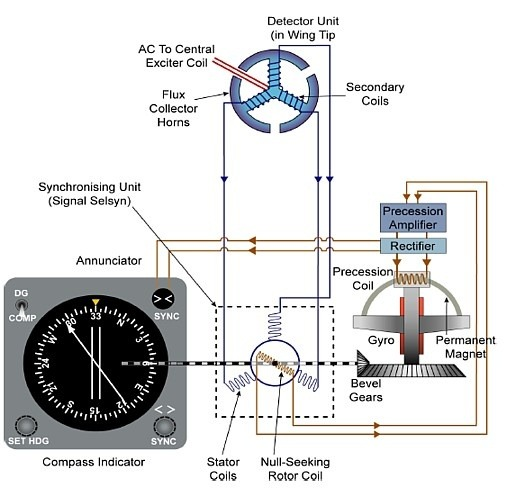
\includegraphics[width=0.7\textwidth]{05.instrumentos.giroscopicos.imagenes/05.05.DGI/05-05-girocompas_esclavo.jpg}

\end{frame}

% \begin{frame}{Girocomp\'as esclavo}

  

% \end{frame}




% \begin{frame}

%   {\tiny Ref: \url{https://www.ecured.cu/Br\%C3\%BAjula_girosc\%C3\%B3pica}}

% \end{frame}